\chapter{Framework \& Methodology}
\label{chap:methodology}

\section{Decentralized Framework Architecture}

The proposed decentralized multi-agent path planning framework is designed to enable each robot to make autonomous decisions based on local observations and communication with nearby agents. The architecture, illustrated in Figure~\ref{fig:framework_architecture} (Adapt the figure number to your actual figure), comprises three main components: a Convolutional Neural Network (CNN) for feature extraction, a Graph Neural Network (GNN) for information aggregation, and a Multi-Layer Perceptron (MLP) for action policy generation.

\begin{figure}[h]
    \centering
    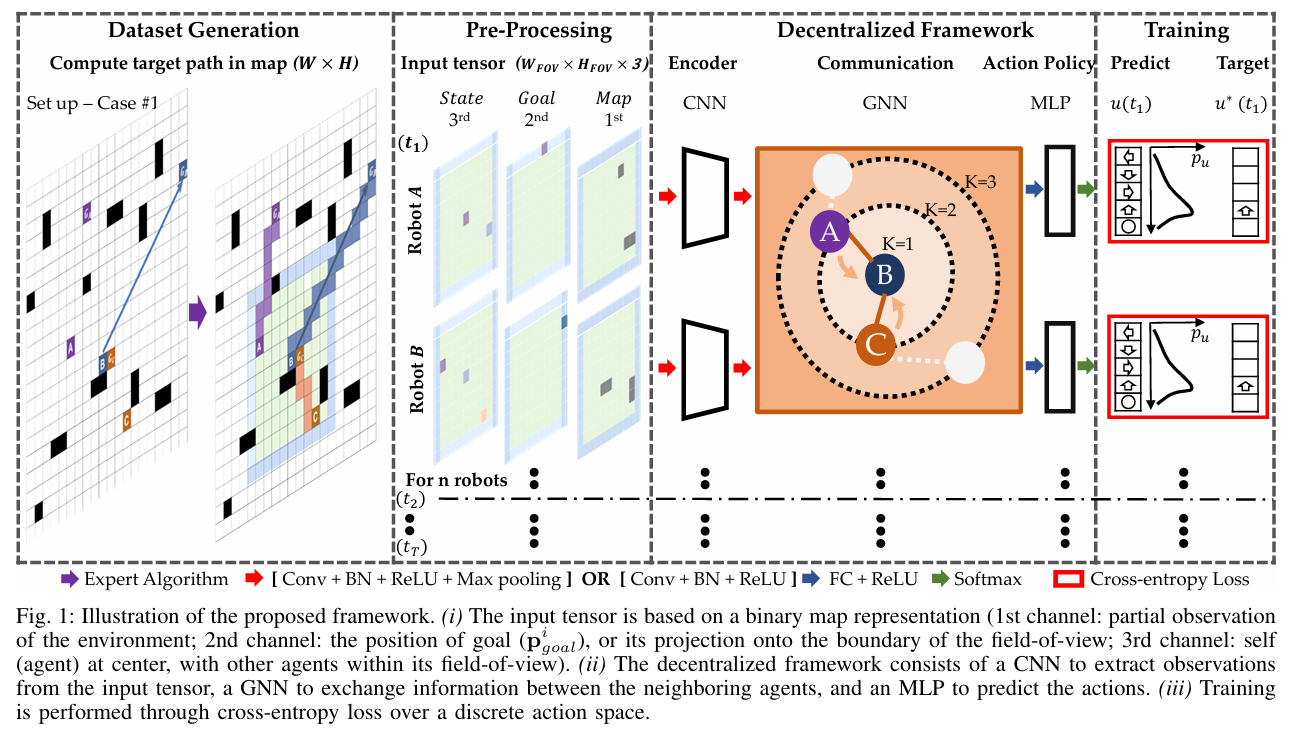
\includegraphics[width=1\textwidth]{images/framework_figure.png} % Replace with your actual figure file and name
    \caption{Decentralized Framework Architecture for Multi-Agent Path Planning}
    \label{fig:framework_architecture}
\end{figure}

\subsection{Observation Processing with Convolutional Neural Network (CNN)}

Each robot is equipped with sensors that provide a local observation of its surroundings, represented as a $W_{FOV} \times H_{FOV} \times 3$ input tensor, as detailed in Chapter~\ref{ch:dataset_generation}. This input tensor is processed by a CNN, which acts as a feature extractor. The CNN is designed to learn relevant features from the local observation map, encoding information about obstacles, goal direction, and nearby agents within a compact feature vector.

The CNN architecture consists of a series of convolutional layers, batch normalization layers, ReLU activation functions, and max-pooling layers.  (Specify the exact layers and configurations of your CNN architecture here, e.g., number of layers, kernel sizes, number of filters, etc. For example:)

\begin{itemize}
    \item \textbf{Convolutional Layer 1:} \textit{X} filters of size \textit{Y}x\textit{Y}, followed by Batch Normalization and ReLU activation.
    \item \textbf{Max-Pooling Layer 1:} Size \textit{Z}x\textit{Z} with stride \textit{S}.
    \item \textbf{Convolutional Layer 2:} \textit{... and so on for each layer}.
\end{itemize}

The output of the CNN is a feature vector $\mathbf{x}_i \in \mathbb{R}^F$ for each robot $i$, summarizing the key information from its local observation. This feature vector serves as the input to the GNN for subsequent information aggregation.

\subsection{Information Aggregation with Graph Neural Network (GNN)}

The GNN component is responsible for enabling communication and information sharing among neighboring robots in a decentralized manner. The multi-robot system is modeled as a dynamic graph $G_t = (V, E_t)$, where each robot $v_i \in V$ is a node, and edges $e_{ij} \in E_t$ represent communication links between robots within a certain communication range $r_{comm}$. The adjacency matrix $S_t$ defines the communication graph at time $t$.

The GNN operates on the feature vectors extracted by the CNNs from all robots. It performs graph convolutions to aggregate information from neighboring robots, allowing each robot to incorporate contextual awareness into its decision-making process.  A single layer GNN is employed, as described in Chapter~\ref{ch:literature_review} and the base paper \cite{Li_et_al_2020}, using the graph convolution operation:

\[
A(X_t; S_t) = \sum_{k=0}^{K-1} S_t^k X_t A_k
\]

where $X_t = [\mathbf{x}_1, \mathbf{x}_2, ..., \mathbf{x}_N]^T \in \mathbb{R}^{N \times F}$ is the matrix of feature vectors from all robots, $S_t$ is the adjacency matrix, $\{A_k\}_{k=0}^{K-1}$ are learnable filter matrices of size $F \times G$, and $K$ is the number of communication hops. The output of the GNN is a matrix $H_t \in \mathbb{R}^{N \times G}$, where each row $\mathbf{h}_i \in \mathbb{R}^G$ represents the aggregated feature vector for robot $i$, incorporating information from its $K$-hop neighbors.

\subsection{Action Policy Generation with Multi-Layer Perceptron (MLP)}

The final component is an MLP, which acts as the action policy network. It takes the aggregated feature vector $\mathbf{h}_i$ from the GNN as input and outputs a probability distribution over a discrete set of actions. In this framework, we consider five discrete actions for each robot: \{'move up', 'move down', 'move left', 'move right', 'idle'\}. The MLP is designed to map the aggregated feature representation to an action that contributes to the robot's goal of reaching its destination while avoiding collisions.

The MLP architecture consists of (Specify the MLP architecture, e.g., number of layers, number of neurons per layer, activation function, etc. For example:)

\begin{itemize}
    \item \textbf{Linear Layer 1:} Input size $G$, Output size \textit{M}, followed by ReLU activation.
    \item \textbf{Linear Layer 2:} Input size \textit{M}, Output size 5 (number of actions), followed by Softmax activation to produce a probability distribution.
\end{itemize}

The action $\mathbf{u}_i$ for robot $i$ is sampled from this probability distribution, representing the robot's chosen action at time $t$.

\section{Imitation Learning Methodology}

The proposed framework is trained using imitation learning, specifically supervised learning with expert demonstrations. The goal of imitation learning is to train the decentralized policy network (CNN-GNN-MLP) to mimic the behavior of the expert algorithm, CBS, which provides optimal or near-optimal path plans.

\subsection{Training Dataset and Loss Function}

The training dataset $\mathcal{T} = \{(\{U^*\}, \{Z\})\}$ consists of pairs of expert action sequences $\{U^*\}$ and corresponding observation sequences $\{Z\}$, generated as described in Chapter~\ref{ch:dataset_generation}. For each scenario in the training set, CBS provides a sequence of optimal actions $U^* = \{U^*_1, U^*_2, ..., U^*_{TMP^*}\}$ for all robots over time steps $t = 1, 2, ..., TMP^*$, where $TMP^*$ is the makespan of the expert solution. Simultaneously, the corresponding observation maps $\{Z\} = \{Z_1, Z_2, ..., Z_{TMP^*}\}$ are recorded.

The model is trained to minimize the cross-entropy loss between the predicted action distribution and the expert action at each time step and for each robot. The loss function is defined as:

\[
\mathcal{L}(\Theta) = \sum_{(\{U^*\}, \{Z\}) \in \mathcal{T}} \sum_{t=1}^{TMP^*} \sum_{i=1}^{N} L_{CE}(\mathbf{u}^*_{i,t}, \pi_{\Theta}(\{Z_t\}, G_t))
\]

where $\Theta$ represents the learnable parameters of the CNN, GNN (filter matrices $\{A_k\}$), and MLP, $\mathbf{u}^*_{i,t}$ is the expert action for robot $i$ at time $t$, and $\pi_{\Theta}(\{Z_t\}, G_t)$ is the action probability distribution predicted by the framework for the observation maps $\{Z_t\}$ and communication graph $G_t$ at time $t$. $L_{CE}$ denotes the cross-entropy loss function.

\subsection{Training Procedure}

The training procedure involves the following steps:

\begin{enumerate}
    \item \textbf{Initialization:} Initialize the parameters $\Theta$ of the CNN, GNN, and MLP networks randomly.
    \item \textbf{Forward Pass:} For each scenario in the training dataset and for each time step $t$:
        \begin{enumerate}
            \item Construct input tensors $\{Z_t\}$ for all robots from the observation maps.
            \item Compute feature vectors $\{\mathbf{x}_{i,t}\}$ using the CNN for each robot.
            \item Construct the adjacency matrix $S_t$ based on robot positions at time $t$.
            \item Aggregate information using the GNN to obtain aggregated feature vectors $\{\mathbf{h}_{i,t}\}$.
            \item Generate action probability distributions $\{\pi_{\Theta}(\{Z_t\}, G_t)\}$ using the MLP for each robot.
        \end{enumerate}
    \item \textbf{Loss Calculation:} Calculate the cross-entropy loss $\mathcal{L}(\Theta)$ between the predicted action distributions and the expert actions $\{U^*\}$.
    \item \textbf{Backpropagation and Optimization:} Compute the gradients of the loss function with respect to the parameters $\Theta$ and update the parameters using an optimization algorithm, such as Adam, to minimize the loss.
    \item \textbf{Iteration and Convergence:} Repeat steps 2-4 for multiple epochs over the training dataset until the loss converges and the model performance on a validation set plateaus.
\end{enumerate}

\subsection{Dataset Aggregation with Online Expert (Optional)}

To further improve the training process and address potential failure cases or deadlocks, a dataset aggregation method with an online expert can be optionally employed. This method, inspired by DAgger \cite{Ross_et_al_2011}, involves periodically deploying the current policy and, in case of failures or suboptimal trajectories, querying the expert (CBS) to resolve these cases and augment the training dataset with corrected expert demonstrations. (Describe your dataset aggregation method in detail if you are implementing it, referencing Algorithm 2 from the base paper if relevant).

\section{Decentralized Online Execution and Collision Shielding}

Once the framework is trained, it is deployed for decentralized online path planning. During execution, each robot independently performs the following steps at each time step:

\begin{enumerate}
    \item \textbf{Local Observation:} Obtain the local observation map $Z_t$.
    \item \textbf{Feature Extraction:} Process $Z_t$ through the CNN to extract feature vector $\mathbf{x}_{i,t}$.
    \item \textbf{Communication and Aggregation:} Communicate with neighboring robots to construct the adjacency matrix $S_t$ and aggregate information using the GNN to obtain $\mathbf{h}_{i,t}$.
    \item \textbf{Action Selection:} Generate action probabilities using the MLP and select an action $\mathbf{u}_{i,t}$ based on the policy $\pi_{\Theta}$.
    \item \textbf{Collision Shielding (Safety Mechanism):} Before executing the chosen action, apply collision shielding to prevent collisions with obstacles or other robots. If the selected action would lead to a collision, override it with an 'idle' action. (Describe your collision shielding mechanism in detail, referencing Algorithm 1 from the base paper if relevant).
    \item \textbf{Execution and State Update:} Execute the (potentially shielded) action, update the robot's position, and proceed to the next time step.
\end{enumerate}

This decentralized execution process allows each robot to navigate autonomously, relying only on local information and communication, while the collision shielding mechanism ensures safety by preventing collisions.

\section{Chapter Summary}

This chapter has presented the framework and methodology for decentralized multi-agent path planning. We detailed the CNN-GNN-MLP architecture designed for decentralized decision-making, the imitation learning approach used for training with expert demonstrations from CBS, and the decentralized online execution process with collision shielding. The combination of these components forms a complete framework for enabling efficient and safe decentralized navigation in multi-robot systems. The next chapter will present preliminary results and discuss the implementation details and experimental setup.